\documentclass[10pt]{article}

\usepackage{amsmath}
% \usepackage[amsmath]{ntheorem}
\usepackage{amsfonts}
\usepackage{graphicx}
\usepackage{fullpage}


\newcommand{\funman}{FUNMAN}
\newcommand{\region}{\bf X}
\newcommand{\posregion}{{\region}^+}
\newcommand{\negregion}{{\region}^-}
\newcommand{\irrelevantregion}{{\region}^\oslash}
\newcommand{\point}{{\bf x}}
\newcommand{\model}{{\bf M}}
\newcommand{\query}{{\bf Q}}
\newcommand{\bounds}{{\bf B}}
\newcommand{\parameters}{{\bf p}}
\newcommand{\parameterbox}{{\bf p}^{[]}}
\newcommand{\reals}{{\mathbb{R}}}

\title{\funman Abstraction}
\author{Dan Bryce}
\begin{document}
\maketitle

\section{Stratification Abstraction}
The SIERHD model from the July monthly demo uses the model summarized by the Petrinet diagram in Figure \ref{fig:seirhd}.

\begin{figure}
    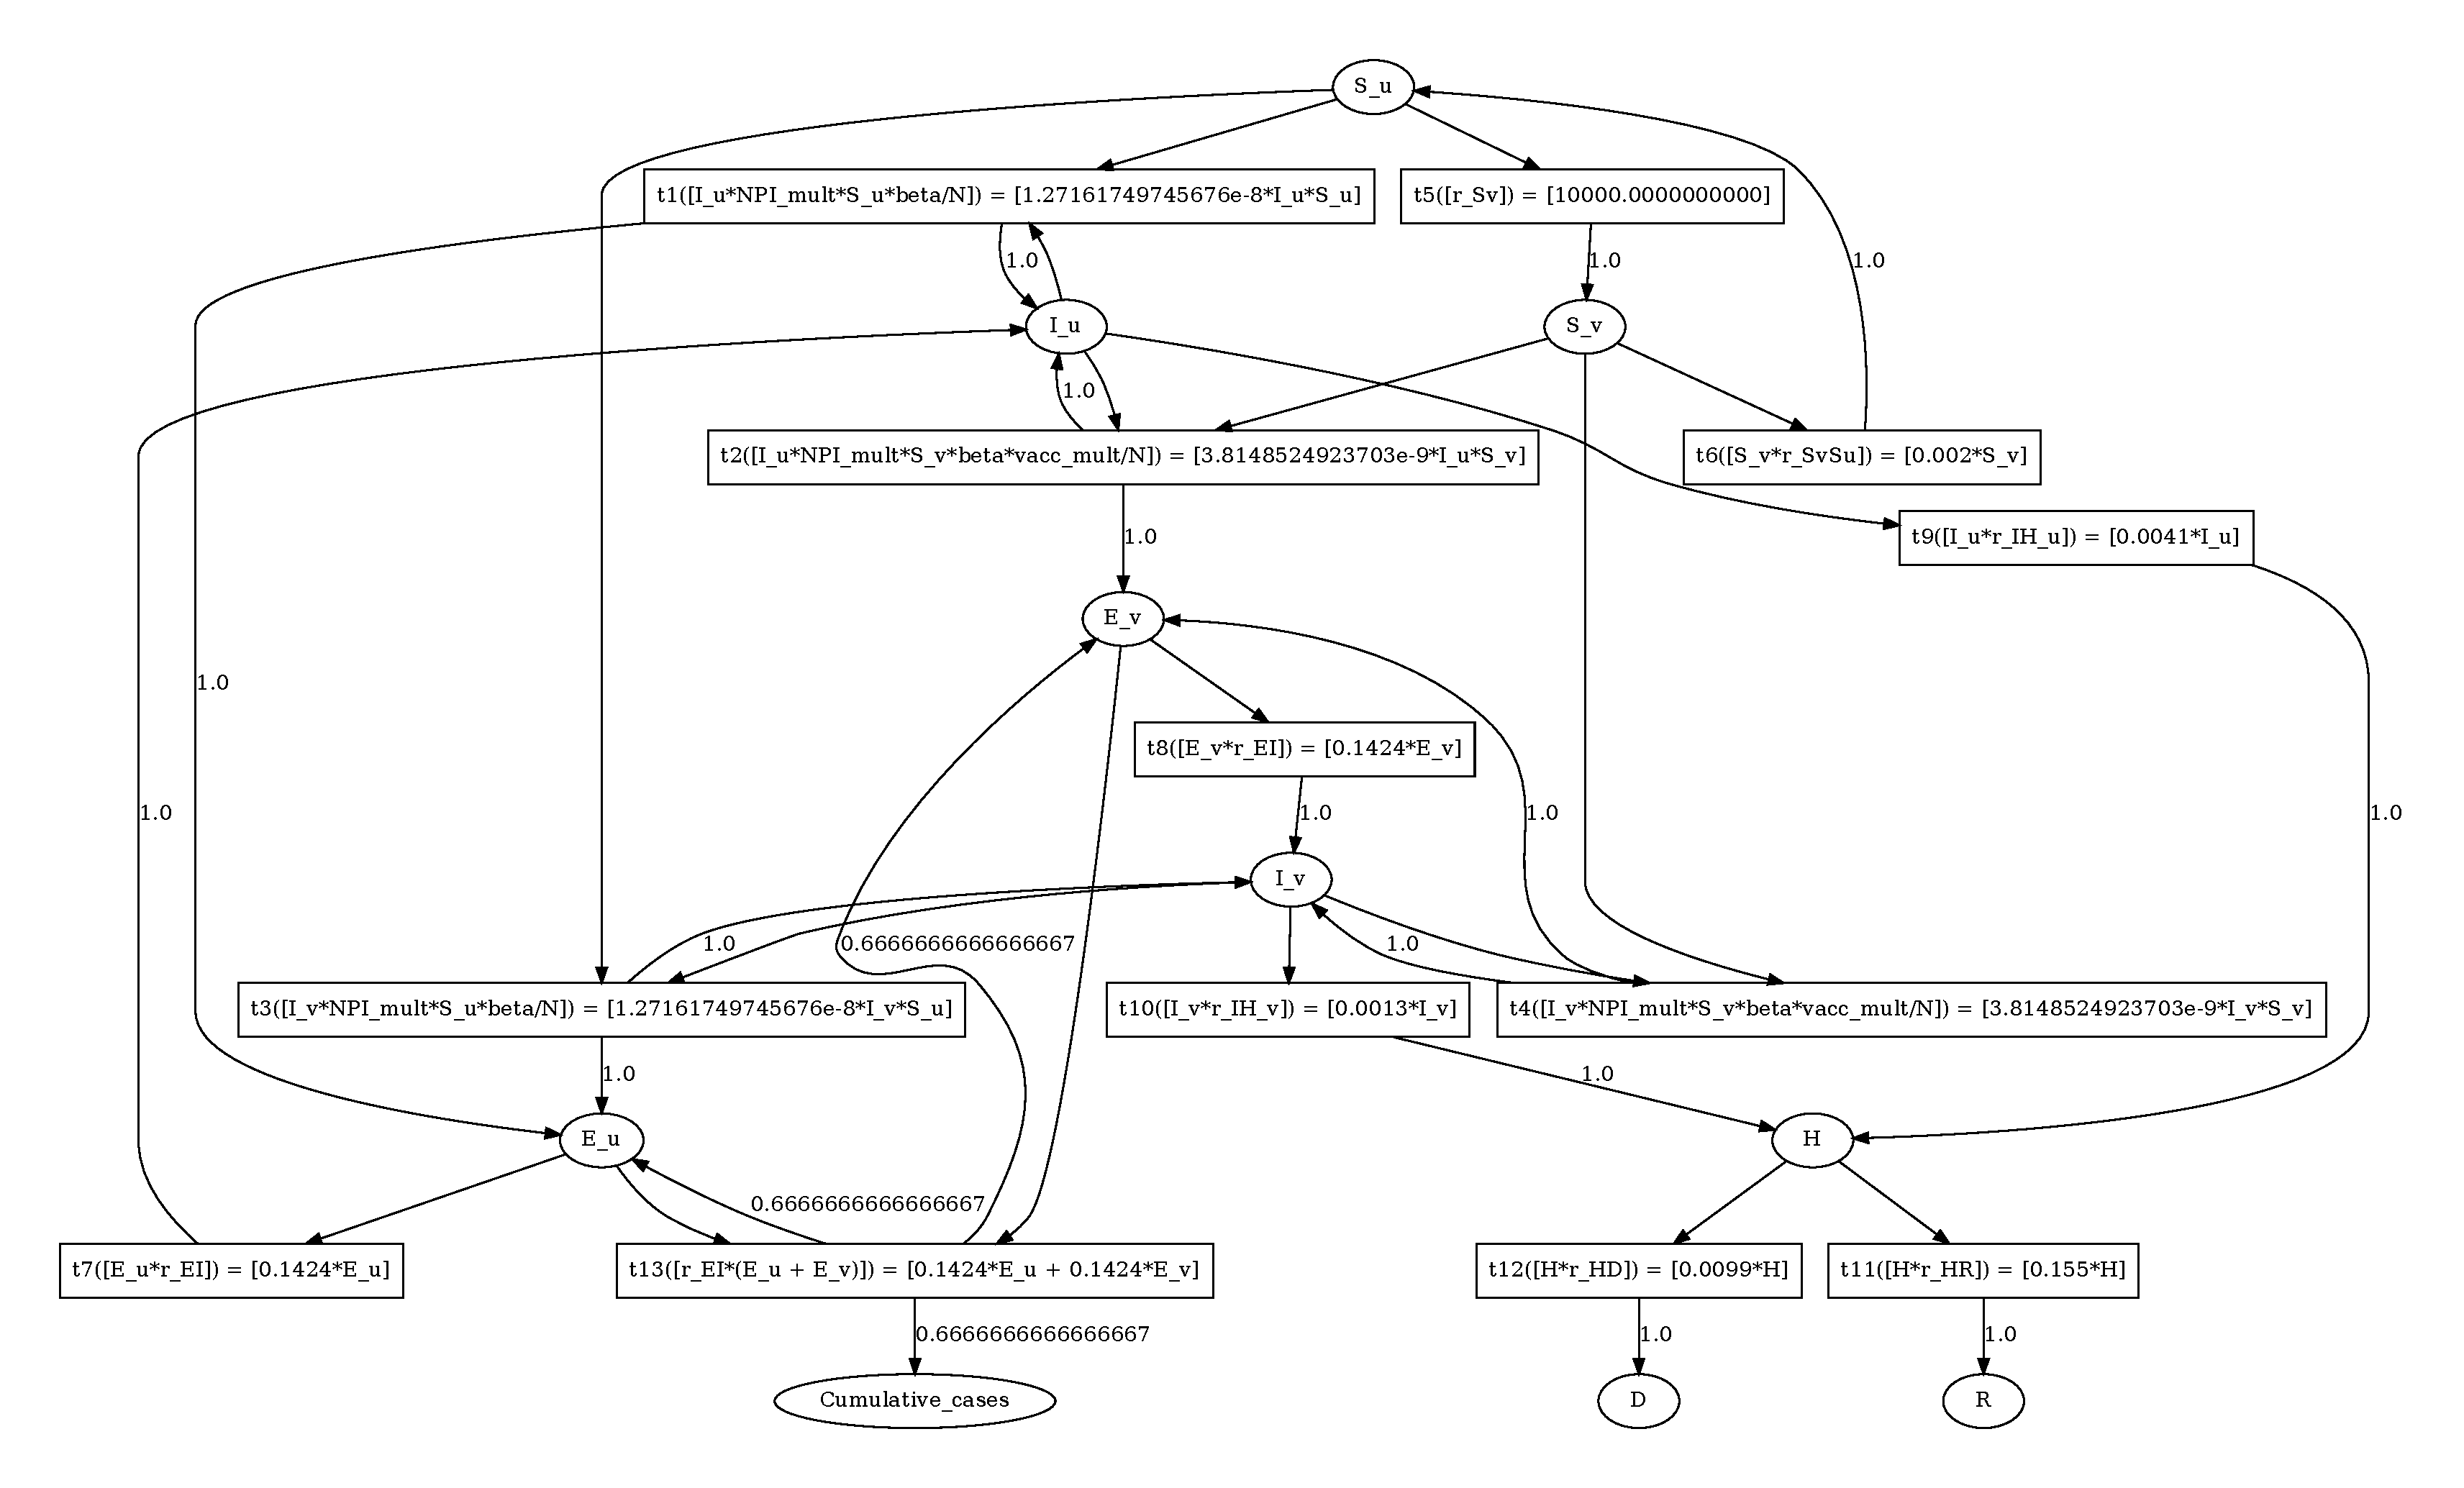
\includegraphics[width=\linewidth]{fig/seirhd}
    \caption{\label{fig:seirhd} SEIRHD Model Petrinet}
\end{figure}

The following transitions connect the variables $S_u$, $S_v$, $E_u$, $E_v$, $I_u$, and $I_v$:

\begin{eqnarray*}
    (I_u, S_u) &\xrightarrow[]{r_1}& (I_u, E_u)\\
    (I_u, S_v) &\xrightarrow[]{r_2}& (I_u, E_v)\\
    (I_v, S_u) &\xrightarrow[]{r_3}& (I_v, E_u)\\
    (I_v, S_v) &\xrightarrow[]{r_4}& (I_v, E_v)\\
    (S_u) &\xrightarrow[]{r_5}& (S_v)\\
    (S_v) &\xrightarrow[]{r_6}& (S_u)\\
    (E_u) &\xrightarrow[]{r_7}& (I_u)\\
    (E_v) &\xrightarrow[]{r_8}& (I_v)
\end{eqnarray*}

Recovering the original, unstratified model corresponds to an abstraction where $S = (S_u, S_v)$, $I = (I_u, I_v)$, and $E = (E_u, E_v)$: 

\begin{eqnarray*}
    (I, S) &\xrightarrow[]{r_1}& (I, E)\\
    (I, S) &\xrightarrow[]{r_2}& (I, E)\\
    (I, S) &\xrightarrow[]{r_3}& (I, E)\\
    (I, S) &\xrightarrow[]{r_4}& (I, E)\\
    (S) &\xrightarrow[]{r_5}& (S)\\
    (S) &\xrightarrow[]{r_6}& (S)\\
    (E) &\xrightarrow[]{r_7}& (I)\\
    (E) &\xrightarrow[]{r_8}& (I)
\end{eqnarray*}

In order for the abstraction to preserve the semantics of the stratified model, it must define $S^t = S_u^t + S_v^t$, $I^t = I_u^t + I_v^t$, and $E^t = E_u^t + E_v^t$ for all time points $t$.  If we look at the definitions for these terms, we have:

\begin{eqnarray*}
    \frac{\partial S_u}{\partial t} &=& - I_u S_u r_1 - I_v S_u r_3 - S_u r_5 + S_v r_6\\
    \frac{\partial S_v}{\partial t} &=& - I_u S_v r_2 - I_v S_v r_4 + S_u r_5 - S_v r_6\\ 
    \frac{\partial S}{\partial t} &=& \frac{\partial S_u}{\partial t}  + \frac{\partial S_v}{\partial t} \\
    &=& - I_u S_u r_1 - I_v S_u r_3 - S_u r_5 + S_v r_6 - I_u S_v r_2 - I_v S_v r_4 + S_u r_5 - S_v r_6\\
    &=& - I_u S_u r_1 - I_v S_u r_3 - I_u S_v r_2 - I_v S_v r_4 \\
\end{eqnarray*}

\begin{eqnarray*}
    \frac{\partial I_u}{\partial t} &=& I_u S_u r_1 - I_u S_u r_1 + I_u S_v r_2 - I_u S_v r_2 + E_u r_7\\
    &=&  E_u r_7\\
    \frac{\partial I_v}{\partial t} &=& I_v S_u r_3 - I_v S_u r_3 + I_v S_v r_4 - I_v S_v r_4 + E_v r_8\\ 
    &=& E_v r_8\\ 
    \frac{\partial I}{\partial t} &=& \frac{\partial I_u}{\partial t}  + \frac{\partial I_v}{\partial t} \\
    &=& E_u r_7 + E_v r_8
\end{eqnarray*}

\begin{eqnarray*}
    \frac{\partial E_u}{\partial t} &=& I_u S_u r_1 + I_v S_u r_3 - E_u r_7\\
    \frac{\partial E_v}{\partial t} &=& I_u S_v r_2 + I_v S_v r_4 - E_v r_8\\ 
    \frac{\partial E}{\partial t} &=& \frac{\partial E_u}{\partial t}  + \frac{\partial E_v}{\partial t} \\
    &=& I_u S_u r_1 + I_v S_u r_3 - E_u r_7 + I_u S_v r_2 + I_v S_v r_4 - E_v r_8
\end{eqnarray*}

Abstraction implies that we allow additional behaviors in the more abstract model (i.e., overapproximate).  In Petrinet models, overapproximation corresponds to cases where the abstract compartment may take on additional values beyond those possible when aggregating the corresponding refined compartments.



\begin{eqnarray*}
    \underline{\frac{\partial S_u}{\partial t}} &\geq&  - \overline{I_u} \overline{S_u} r_1 - \overline{I_v} \overline{S_u} r_3 - \overline{S_u} r_5 + \underline{S_v} r_6\\
    &=&  - N^2 r_1 - N^2 r_3 - N r_5 + 0 r_6\\
    &=&  - S_u^0 (N  r_1 + N r_3 + r_5)\\
    \\
    \overline{\frac{\partial S_u}{\partial t}} &\leq&  - \underline{I_u} \underline{S_u} r_1 - \underline{I_v} \underline{S_u} r_3 - \underline{S_u} r_5 + \overline{S_v} r_6\\
    &=&   - 0 0 r_1 - 0 0 r_3 - 0 r_5 + S_v^0 r_6\\
    &=&  S_v^0 r_6\\
    \\
    \underline{\frac{\partial S_v}{\partial t}} &\geq&  - \overline{I_u} \overline{S_v} r_2 - \overline{I_v} \overline{S_v} r_4 + \underline{S_u} r_5 +-\overline{S_v} r_6\\
    &=&  - N S_v^0 r_1 - N S_v^0 r_4 - 0 r_5 + S_v^0 r_6\\
    &=&  - S_v^0 (N  r_1 + N r_4 + r_6)\\
    \\
    \overline{\frac{\partial S_v}{\partial t}} &\leq&  - \underline{I_u} \underline{S_v} r_2 - \underline{I_v} \underline{S_v} r_4 + \overline{S_u} r_5 -\underline{S_v} r_6\\
    &=&  - 0 0 r_1 -0 0 r_4 + S_u^0 r_5 - 0 r_6\\
    &=&  S_u^0 r_5\\
    \\
    \frac{\partial S}{\partial t} &\leq& \overline{\frac{\partial S_u}{\partial t}}  + \overline{\frac{\partial S_v}{\partial t}}\\
    &\leq& S_v^0 r_6 + S_u^0 r_5\\
    \frac{\partial S}{\partial t} &\geq& \underline{\frac{\partial S_u}{\partial t}}  + \underline{\frac{\partial S_v}{\partial t}}\\
    &\geq& - S_u^0 (N  r_1 + N r_3 + r_5) - S_v^0 (N  r_1 + N r_4 + r_6)
    \\
\end{eqnarray*}

\begin{eqnarray*}
    \underline{\frac{\partial I_u}{\partial t}} &\geq&   \underline{I_u} \underline{S_u} r_1 - \overline{I_u} \overline{S_u} r_1 + \underline{I_u} \underline{S_v} r_2 - \overline{I_u} \overline{S_v} r_2 + \underline{E_u} r_7\\
    &=&  0 0 r_1 - N S_u^0 r_1 + 0 0 r_2 - N S_v^0 r_2 + 0 r_7\\
    &=&  - N (S_u^0 r_1 + S_v^0 r_2)\\
    \\
    \overline{\frac{\partial I_u}{\partial t}} &\leq& \overline{I_u} \overline{S_u} r_1 - \underline{I_u} \underline{S_u} r_1 + \overline{I_u} \overline{S_v} r_2 - \underline{I_u} \underline{S_v} r_2 + \overline{E_u} r_7\\
    &=&  N S_u^0 r_1 - 0 0 r_1 + N S_v^0 r_2 - 0 0 r_2 + N r_7\\
    &=&  N (S_u^0 r_1 + S_v^0 r_2 + r_7)\\
    \\
    \underline{\frac{\partial I_v}{\partial t}} &\geq&  \underline{I_v} \underline{S_u} r_3 - \overline{I_v} \overline{S_u} r_3 + \underline{I_v} \underline{S_v} r_4 - \overline{I_v} \overline{S_v} r_4 + \underline{E_v} r_8\\
    &=&  0 0 r_3 - N S_u^0 r_3 + 0 0  r_4 - N S_v^0 r_4 + 0 r_8\\
    &=&  - N (S_u^0 r_3 + S_v^0 r_4)\\
    \\
    \overline{\frac{\partial I_v}{\partial t}} &\leq&  \overline{I_v} \overline{S_u} r_3 - \underline{I_v} \underline{S_u} r_3 + \overline{I_v} \overline{S_v} r_4 - \underline{I_v} \underline{S_v} r_4 + \overline{E_v} r_8\\
    &=&  N S_u^0 r_3 - 0 0 r_3 + N S_v^0 r_4 - 0 0 r_4 + N r_8\\
    &=&  N (S_u^0 r_3 + S_v^0 r_4 + r_8)\\
    \\
    \frac{\partial I}{\partial t} &\leq& \overline{\frac{\partial I_u}{\partial t}}  + \overline{\frac{\partial I_v}{\partial t}}\\
    &\leq& N (S_u^0 r_1 + S_v^0 r_2 + r_7) + N (S_u^0 r_3 + S_v^0 r_4 + r_8)\\
    &=& N (S_u^0 r_1 + S_v^0 r_2 + r_7 + S_u^0 r_3 + S_v^0 r_4 + r_8)\\
    \frac{\partial I}{\partial t} &\geq& \underline{\frac{\partial I_u}{\partial t}}  + \underline{\frac{\partial I_v}{\partial t}}\\
    &\geq& - N (S_u^0 r_1 + S_v^0 r_2 + S_u^0 r_3 + S_v^0 r_4)
    \\
\end{eqnarray*}

\begin{eqnarray*}
    \underline{\frac{\partial E_u}{\partial t}} &\geq&   \underline{I_u} \underline{S_u} r_1 + \underline{I_v} \underline{S_u} r_3 - \overline{E_u} r_7\\
    &=&  0 0  r_1 + 0 0 r_3 - N r_7\\
    &=&  - N r_7\\
    \\
    \overline{\frac{\partial E_u}{\partial t}} &\leq& \overline{I_u} \overline{S_u} r_1 + \overline{I_v} \overline{S_u} r_3 - \underline{E_u} r_7\\
    &=&  N S_u^0 r_1 + N S_u^0 r_3 - 0 r_7\\
    &=&  N S_u^0 (r_1 + r_3)\\
    \\
    \underline{\frac{\partial E_v}{\partial t}} &\geq&  \underline{I_u} \underline{S_v} r_2 + \underline{I_v} \underline{S_v} r_4 - \overline{E_v} r_8\\
    &=&  0 0 r_2 + 0 0  r_4 -N r_8\\
    &=&  -N r_8\\
    \\
    \overline{\frac{\partial E_v}{\partial t}} &\leq&  \overline{I_u} \overline{S_v} r_2 + \overline{I_v} \overline{S_v} r_4 - \underline{E_v} r_8\\
    &=&  N S_v^0 r_2 +N S_v^0 r_4 - 0 r_8\\
    &=&  N S_v^0 (r_2 + r_4)\\
    \\
    \frac{\partial E}{\partial t} &\leq& \overline{\frac{\partial E_u}{\partial t}}  + \overline{\frac{\partial E_v}{\partial t}}\\
    &\leq& N S_u^0 (r_1 + r_3) +N S_v^0 (r_2 + r_4)\\
    \frac{\partial E}{\partial t} &\geq& \underline{\frac{\partial E_u}{\partial t}}  + \underline{\frac{\partial E_v}{\partial t}}\\
    &\geq& - N (r_7 + r_8)\\
    \\
\end{eqnarray*}

\begin{eqnarray*}
    S^{t+dt} &=& S^t + \frac{\partial S}{\partial t}dt\\
    S^{t+dt} &\leq& S^t + \overline{\frac{\partial S}{\partial t}}dt\\
    &=& S^t + (- \underline{I_u} \underline{S_u} r_1 - \underline{I_v} \underline{S_u} r_3 - \underline{S_u} r_5 + \overline{S_v} r_6)dt
\end{eqnarray*}

Assume that all compartments are population constrained.  Use information about monotonicity.

\[\frac{\partial S_u}{\partial t} \leq 0, 0 \leq S_u \leq N\]
\[\frac{\partial S_v}{\partial t} \leq 0, 0 \leq S_v \leq N\]
\[ 0 \leq I_u \leq N\]
\[ 0 \leq I_v \leq N\]

% \section{Parameter Synthesis as Abstraction Refinement}

% Parameter synthesis involves labeling regions of a parameter space as safe or unsafe.  This can be formulated as an expression:

% \begin{align}
%     \label{eqn:formulation1}\tag{F1}
%      & \exists \posregion \subseteq \reals^n \forall \point \in \posregion. \model(\point) \wedge \query(\point)         & // & \text{true}  \\
%     \label{eqn:formulation2}\tag{F2}
%      & \exists \negregion \subseteq \reals^n \forall \point \in \negregion. \neg \model(\point) \vee \neg \query(\point) & // & \text{false}
%     % \label{eqn:formulation3}
%     %  & \exists \irrelevantregion \subseteq \reals^n \forall \point \in \irrelevantregion. \neg \model(\point)         & // & \text{irrelevant}
% \end{align}
% \noindent where each point $\point$ is an $n$-dimensional vector.  We refer to $\posregion$ and $\negregion$ as the respective ``true'' and ``false'' sets.  We call the pair $(\posregion, \negregion)$ the parameter space of $\model$ and $\query$.



% In addition to the parameters comprising the parameter space, the model includes a set of state variables $V$.  The model defines (via ODE or PDE equations) the state $S$ at various points in time and space.  We augment the state to include the (constant or piece-wise constant) model parameters, as well as structural parameters describing the time horizon and step size.

% An abstraction of the state space groups states into abstract states, and defines abstract transitions between abstract states.  An abstract transition between abstract states indicates that there exists at least one transition between states of the respective abstract states.  

\end{document}